\documentclass[9pt]{beamer}

\usepackage{beamerpreamble}
\usepackage[swedish]{babel}
\usepackage{minted}
\usepackage{comment}
\usemintedstyle{vs}

\usepackage{tikz}

\renewcommand{\ttdefault}{cmtt}

\newcommand*\mean[1]{\bar{#1}}

\title{Mätvärdesbehandling}
\author[benjamin.eriksson@physics.uu.se]{Benjamin Eriksson  \\ \vspace{0.5cm} \scriptsize{Slides av M. Isacson} \\ \tiny{med inspiration från} \\ \scriptsize{M. Ellert, M. Olvegård, och B. Lindgren}}
\institute[Uppsala universitet]{{\small Avdelningen för tillämpad kärnfysik \\ Institutionen för fysik och astronomi} \\ \uulogo}
\date{{\small Reviderad}\\ \today}

\begin{document}
    \frame{\titlepage}

    \begin{frame}
        Studentportalen/DOKUMENT/Laborationer/Datorlabb
        \begin{itemize}
            \item matvarden.pdf (denna föreläsning)
            \item Kompendium.pdf
            \item Sammanfattning.pdf
            \item lektionsuppgift.pdf
        \end{itemize}

        \vfill

        Lektionsuppgiften består av 4 uppgifter. Gör de i ordning! Uppgift 1 är den
        viktigaste då den relaterar till Labb 4 (samt kommande kurser) men försök
        också hinna med 2 och 3. Uppgift 4 görs endast i mån av tid. \emph{Fråga om ni kör fast!}

        \vfill

        Men först några ord om mätvärdesbehandling...
    \end{frame}


   

    \begin{frame}
        \onslide<+->
        Säg att ni från slumpvariabeln $X$ erhållit mätserien $\{x_i\}_1^n$. Viktiga frågor är då

        \begin{enumerate}
            \item Vad är det förväntade värdet för en mätning $x_i$?
            \item Hur stor är spridningen hos mätvärdena?
            \item Hur väl kan vi skatta det sanna väntevärdet av slumpvariabeln $X$?
        \end{enumerate}

        \vfill

        \begin{columns}[T]
            \column{.6\textwidth}
            \onslide<+->{
            \begin{enumerate}
                \item Medelvärdet: $\mean{x} = \frac1n \sum_{i=1}^n x_i$
                    \begin{itemize}
                        \item $\mean{x}$ skattar väntevärdet $\mu=E[x]$.
                    \end{itemize}
                \item Standardavvikelse: \\
                    \vspace{0.5em}
                    $u(x) = \sqrt{\frac1{n-1} \sum_{i=1}^n \left(x_i - \mean{x}\right)^2}$
                    \vspace{0.5em}
                    \begin{itemize}
                        \item $u(x)$ är ett mått på spridningen av mätvärdena $x_i$ och skattar den sanna standardavvikelsen $\sigma$.
                    \end{itemize}
                \item Standardosäkerhet i medelvärdet: \\
                    \vspace{0.5em}
                    $u(\mean{x}) = \frac{u(x)}{\sqrt{n}} = \sqrt{\frac1{n(n-1)} \sum_{i=1}^n \left(x_i - \mean{x}\right)^2}$
                    \vspace{0.5em}
                    \begin{itemize}
                        \item $u(\mean{x})$ skattar \emph{spridningen i medelvärdet} vi skulle få om experimentet upprepades flera gånger.
                    \end{itemize}
            \end{enumerate}
            }
            \column{.4\textwidth}
            \hspace{-0.2\textwidth}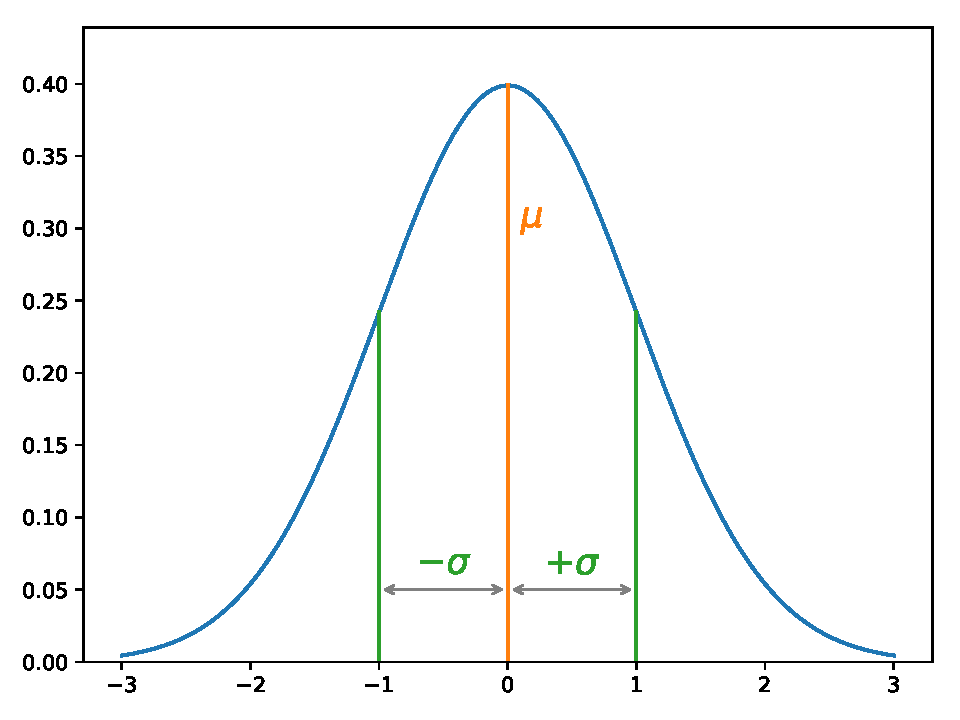
\includegraphics[width=1.2\textwidth]{gaus.pdf}
        \end{columns}
    \end{frame}

    \begin{frame}[fragile]
        Matlabexempel:
        \begin{minted}[frame=leftline,framesep=2mm,autogobble,escapeinside=||]{matlab}
        % generera 1000 mätvärden |$x_i$| med |$\mu=0$| och |$\sigma=1$|
        x = normrnd(0, 1, 1, 1000);
        m = mean(x); % medelvärde |$\bar{x}=0.012431$|
        u = std(x); % standardavvikelse |$u(x)=0.973136$|

        % standardosäkerhet i medelvärdet
        um = u/sqrt(length(x)); % |$u(\bar{x})=0.030773$|

        % upprepa experimentet 500 gånger
        means = zeros(1, 500);
        for i=1:length(means)
        % generera 1000 mätvärden x_i med mu=0 och sigma=1
            x = normrnd(0, 1, 1, 1000);
            means(i) = mean(x); % beräkna medelvärdet
        end

        % spridningen i medelvärdet från många experiment
        umeans = std(means); % |$u(\bar{x})=0.031604$|
        \end{minted}

    \end{frame}

    

    \begin{frame}
        Exempel:
        \begin{gather*}
            x_1 = \SI{0.97}{m}\\
            x_2 = \SI{1.09}{m}\\
            x_3 = \SI{1.16}{m}\\
            x_4 = \SI{1.04}{m}\\
            x_5 = \SI{1.12}{m}
        \end{gather*}

        \begin{enumerate}
            \item Beräkna medelvärdet
            \item Beräkna standardavvikelsen
            \item Beräkna standardosäkerheten i medelvärdet
            \item Ange medelvärdet med dess osäkerhet
        \end{enumerate}

        \end{frame}
        \begin{frame}

            \begin{enumerate}
                \item<+-> Medelvärdet:
                    \begin{equation*}
                        \mean{x} = \frac15 \sum_{i=1}^5 x_i = \frac{0.97 + 1.09 + 1.16 + 1.04 + 1.12}{5} = \SI{1.08}{m}
                    \end{equation*}

                \item<+-> Standardavvikelsen:
                    \begin{gather*}
                        u(x) = \sqrt{\frac1{5-1} \sum_{i=1}^5 \left(x_i - \mean{x}\right)^2} \\= \sqrt{\frac{(0.97 - 1.08)^2 + (1.09 - 1.08)^2 + (1.16 - 1.08)^2 + (1.04 - 1.08)^2 + (1.12 - 1.08)^2}{5-1}} \\= \SI{0.07}{m}
                    \end{gather*}

                \item<+-> Standardosäkerheten i medelvärdet:
                    \begin{equation*}
                        u(\mean{x}) = \frac{0.07}{\sqrt5} = \SI{0.03}{m}
                    \end{equation*}

                \item<+-> $\mean{x} = \SI{1.08\pm0.03}{m} = \SI[separate-uncertainty=true]{1.08\pm0.03}{m}$
            \end{enumerate}
    \end{frame}

    \begin{frame}[fragile]
        I Matlab:

        \begin{minted}[frame=leftline,framesep=2mm,autogobble]{matlab}
            % mätdata
            x = [0.97, 1.09, 1.16, 1.04, 1.12]

            % medelvärdet
            m = mean(x)

            % standardavvikelsen, u(x)
            s = std(x)

            % standardosäkerheten i medelvärdet, u(m)
            sm = std(x)/sqrt(length(x))
        \end{minted}
    \end{frame}

    \begin{frame}
        Hur många värdesiffor ska vi ange i svaret?

        \vfill

        \hrule\vspace{0.4em}
        Allmänna regler: \\
        Vid $\times$ och $\div$ ges antalet \emph{värdesiffror} av faktorn med \emph{minst} antal värdesiffror
        \begin{gather*}
            \textcolor{blue}{1.3}\times1434\times5.10432 = \textcolor{blue}{9.5}\times10^3\\
            431.5\times1.52 / \textcolor{blue}{5.4} = \textcolor{blue}{12}
        \end{gather*}
        Vid $+$ och $-$ ges antalet \emph{decimaler} av termen med \emph{störst} osäkerhet
        \begin{equation*}
            11.\textcolor{blue}{45} + 1.421 - 6.9321 = 5.\textcolor{blue}{94}
        \end{equation*}
        \hrule

        \vfill

        Vi kommer dock nöja oss med följande \textbf{tumregel}:
        \begin{itemize}
            \item Avrunda osäkerheten till \textcolor{red}{\textbf{två värdesiffror}} och justera mätetalet därefter.
        \end{itemize}

        \vfill
        Exempel: Om beräkningar ger $\mean{x} = 22.1572$ och $u(\mean{x}) = 0.4217$ ska detta skrivas som
                \begin{equation*}
                    \mean{x}=\num{22.16\pm0.42} \quad \text{eller} \quad \mean{x}=\num[separate-uncertainty=true]{22.16\pm0.42}
                \end{equation*}
    \end{frame}

    \begin{frame}
        \begin{center}
            \huge{Minstakvadratmetoden}
        \end{center}
    \end{frame}

    \begin{frame}
        Vi är oftast intresserade av \emph{funktionella samband} mellan två
        eller flera storheter. Säg att vi har en storhet $y$ som i sin tur beror på en annan storhet $x$.

        \begin{itemize}
            \item Position $s$ som beror av en tid $t$
            \item Ström $I$ beroende av en pålagd spänning $V$
            \item Periodtid $T$ beroende av pendelarm $L$
            \item \ldots
        \end{itemize}

        Genom att variera $x$ och mäta $y$ fås två mätserier $\{x_i\}_1^n$ och
        $\{y_i\}_1^n$, alternativ en mätserie av paren $\{x_i,y_i\}_1^n$.

        \vfill
        \begin{columns}
            \column{.5\textwidth}
            Hur finner vi sambandet $y=f(x)$ med hjälp av dessa mätningar?
            \column{.5\textwidth}
            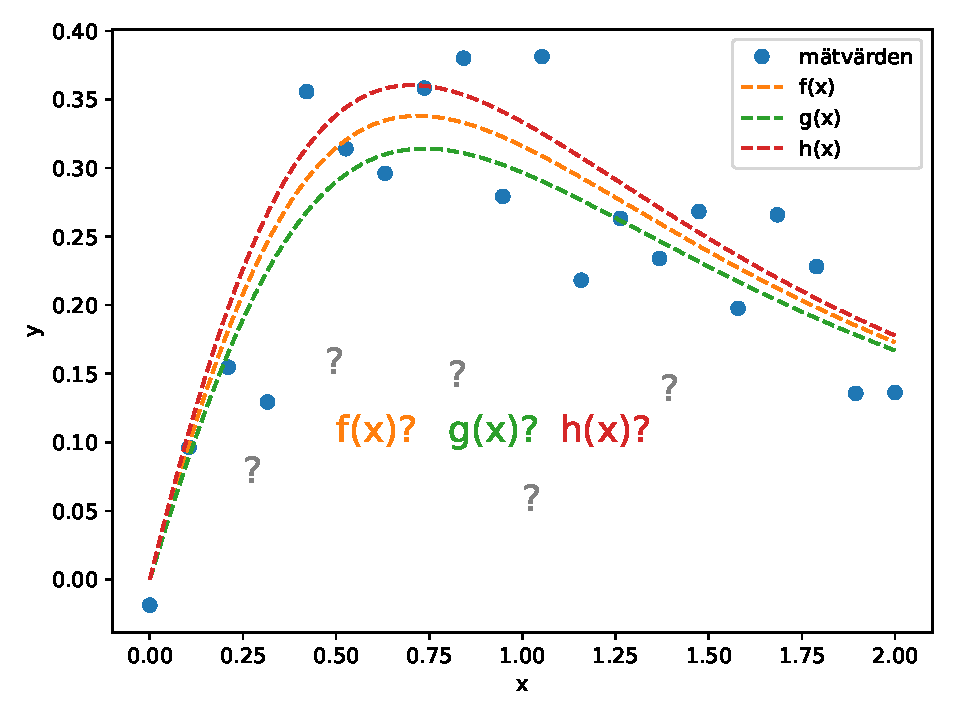
\includegraphics[width=\textwidth]{anpassning0.pdf}
        \end{columns}
    \end{frame}

    \begin{frame}
        Sambandet $f$ kan t.ex. vara en teoretisk modell beroende på ett antal parameterar $a_j$, dvs
        \begin{equation*}
            y = f(x,a_1, a_2, \ldots, a_m)
        \end{equation*}

        \vfill

        \begin{columns}[C]
            \column{.5\textwidth}
            Hur bra beskriver $f$ vår mätdata $\{x_i,y_i\}$? Bilda kvadratsumman $S$:
            \begin{equation*}
                S = \sum_i\left(y_i - f(x_i,a_1,\ldots,a_m)\right)^2
            \end{equation*}
            $\rightarrow$ Ju mindre skillnad mellan $y_i$ och $f(x_i)$ desto mindre blir $S$.

            \column{.5\textwidth}
            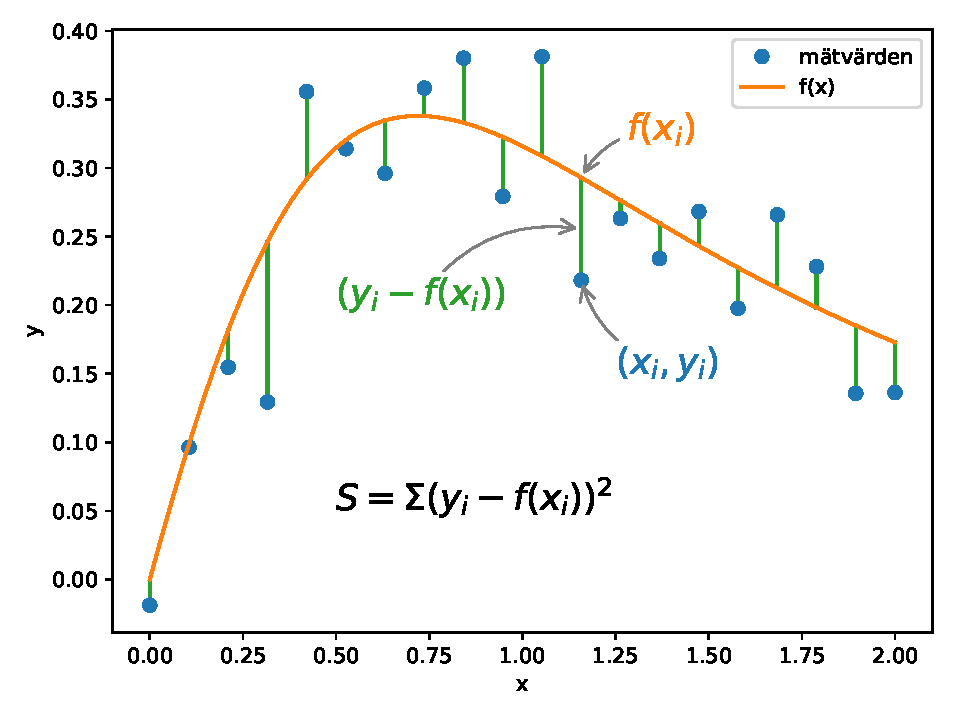
\includegraphics[width=\textwidth]{S.pdf}
        \end{columns}

        \vfill
        Vi kan alltså \emph{minimera} $S$ med avseende på parametrarna $a_j$ för
        att få den bästa anpassningen till vår mätdata! Detta kallas för
        \emph{minstakvadratanpassing}.

        \begin{equation*}
            \frac{\partial S}{\partial a_1} = 0,
            \frac{\partial S}{\partial a_2} = 0,\quad\ldots,
            \frac{\partial S}{\partial a_m} = 0
        \end{equation*}
        Observera att derivatorna tas med avseende på parametrarna $a_j$ (\textbf{inte} mätvärdena)!
    \end{frame}



    \begin{frame}
        Exempel: Anpassa en linje $y=a_1x + a_2$ till en mätserie $\{x_i, y_i\}$.
        \begin{columns}[T]
            \column{.5\textwidth}
            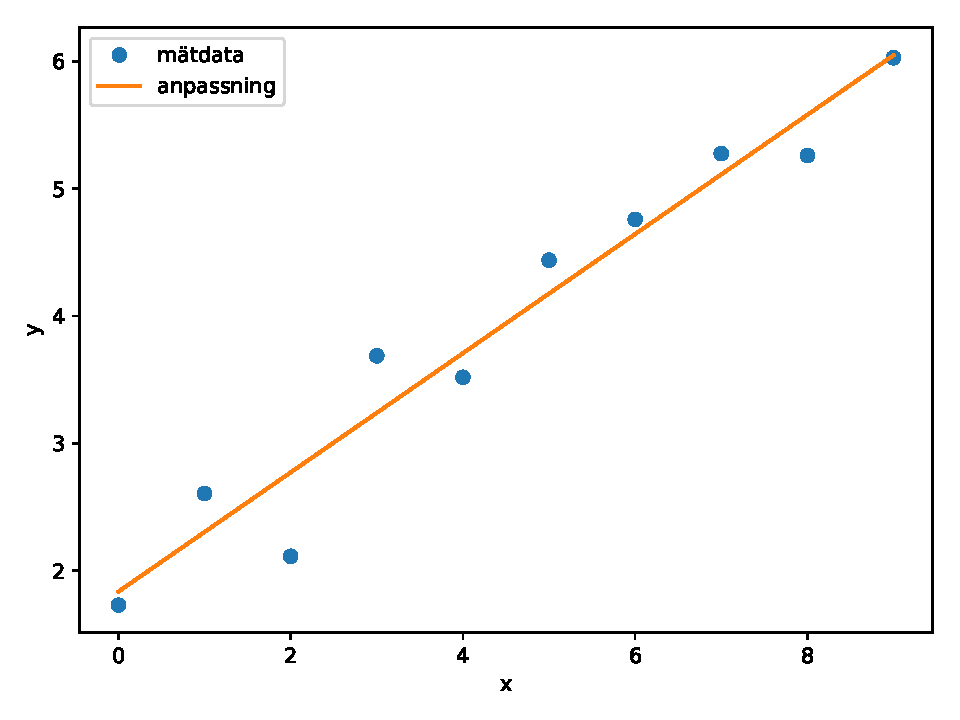
\includegraphics[width=\textwidth]{anpassning2.pdf}
            \column{.5\textwidth}
            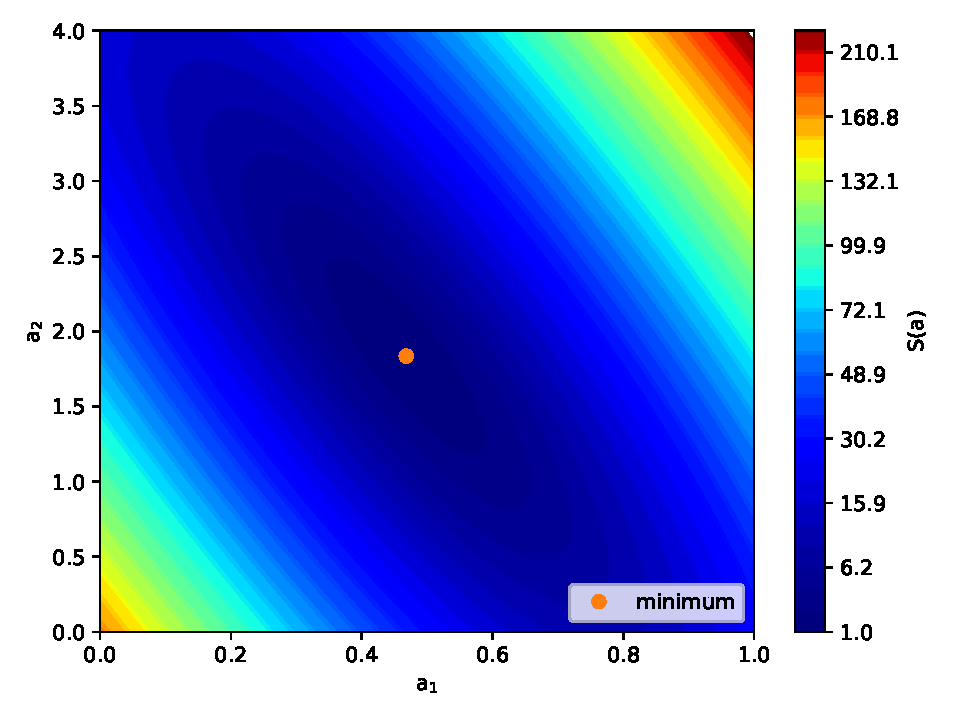
\includegraphics[width=\textwidth]{s2.pdf}
        \end{columns}

        Bilda kvadratsumman $S$:
        \begin{equation*}
            S(a_1, a_2) = \sum_i (y_i - f(x_i,a_1,a_2))^2 = \sum_i (y_i - a_1x_i - a_2)^2
        \end{equation*}
        $S$ är nu en funktion av två variabler, $a_1$ och $a_2$, och måste minimeras över båda!
    \end{frame}

    \begin{frame}
        \onslide<+->
        De partiella derivatorna är då:
        \begin{align*}
            \frac{\partial S}{\partial a_1} &= -2\sum_i(y_i - a_1x_i - a_2)x_i = -2\left(\sum_i y_ix_i - \sum_i a_1 x_i^2 - \sum_i a_2 x_i\right) = 0 \\
            \frac{\partial S}{\partial a_2} &= -2\sum_i (y_i - a_1x_i - a_2) = -2\left(\sum_i y_i - \sum_i a_1x_i - \sum_i a_2\right)= 0 \\
        \end{align*}
        \onslide<+->
        Och om vi arrangerar om termerna:
        \begin{align*}
            \sum_i y_ix_i &= a_1 \sum_i x_i^2 + a_2 \sum_i x_i \\% = a_0 \sum_i x_i + a_1\sum_ix_i^2 \\
            \sum_i y_i &= a_1 \sum_i x_i + a_2 \sum_i 1 \\ %= na_0 + a_1\sum_i x_i \\
        \end{align*}
        Detta är ett \emph{linjärt ekvationssystem} i variablerna $a_1$ och $a_2$,
        som kan skrivas om på matrisform (notera $\sum_i 1 = n$):
        \begin{equation*}
            \begin{pmatrix}
                \sum_i y_ix_i \\
                \sum_i y_i
            \end{pmatrix} =
            \begin{pmatrix}
                \sum_i x_i^2 & \sum_ix_i \\
                \sum_i x_i  & n \\
            \end{pmatrix}
            \begin{pmatrix}
                a_1 \\
                a_2
            \end{pmatrix}
        \end{equation*}
    \end{frame}

    \begin{frame}[fragile]
        Om vi sätter
        \begin{equation*}
            \vec h =
            \begin{pmatrix}
                \sum_i y_ix_i \\
                \sum_i y_i
            \end{pmatrix},\quad
            G =
            \begin{pmatrix}
                \sum_i x_i^2 & \sum_ix_i \\
                \sum_i x_i & n
            \end{pmatrix},\quad
            \vec a =
            \begin{pmatrix}
                a_1 \\
                a_2
            \end{pmatrix}
        \end{equation*}
        kan detta skrivas som $G\vec a = \vec h$ och allt vi behöver göra är att lösa för $\vec a$:
        \begin{equation*}
            \vec a = G^{-1}\vec h
        \end{equation*}

        I Matlab:
        \begin{minted}[frame=leftline,framesep=2mm,autogobble,escapeinside=||]{matlab}
            x = [|\ldots|]; y = [|\ldots|]; % mätdata |$\{x_i, y_i\}$|
            G = [sum(x.^2), sum(x); sum(x), length(x)]; % matrisen |$G$|
            h = [sum(y.*x); sum(y)]; % högerledet |$h$|
            a = inv(G)*h % de anpassade parametrarna |$a = (a_1, a_2)^\top$|
        \end{minted}

        \vfill
        I det exemplet fås $a_1 = 0.47$ och $a_2 = 1.84$, jmf sanna värdena $a_1 = 0.50$ och $a_2 = 1.70$.
    \end{frame}

    \begin{frame}[fragile]
        Eftersom våra mätvärden $\{x_i, y_i\}$ har en viss spridning finns det
        en osäkerhet i de anpassade parametrarna $\vec a = (a_1,\ldots,a_j,\ldots,a_m)^\top$. Denna ges av
        \begin{equation*}
            u(a_j) = \sqrt{\frac{(G^{-1})_{jj}S}{n - m}}
        \end{equation*}
        där
        \begin{itemize}
            \item $(G^{-1})_{jj}$ är diagonalelementen i $G^{-1}$,
            \item $S=\sum_i(y_i - f(x_i,\vec a))^2$ är kvadratsumman som tidigare,
            \item $n$ är antalet mätpunkter och $m$ är antalet anpassade parametrar.
                \begin{itemize}
                    \item $n-m$ kallas för antalet \emph{frihetsgrader} och betecknas $\nu = n - m$.
                \end{itemize}
        \end{itemize}

        \vfill
        I Matlab:
        \begin{minted}[frame=leftline,framesep=2mm,autogobble,escapeinside=||]{matlab}
            a = inv(G)*h % de anpassade parametrarna |$a = (a_1,\ldots,a_m)^\top$|
            S = sum((y-f(x,a)).^2); % kvadratsumman |$S(a) = \sum(y_i - f(x_i, a))^2$|
            n = length(x); m = length(a); % #mätvärden |$n$| och #parametrar |$m$|

            % vektor med mätosäkerheterna |$u_a = (u_{a_1},\ldots,u_{a_m})^\top$|
            ua = sqrt(diag(inv(G))*S/(n - m));
        \end{minted}
    \end{frame}

    \begin{frame}[fragile]
        Komplett matlab-exempel för vår räta linje:

        \begin{minted}[frame=leftline,framesep=2mm,autogobble,escapeinside=||]{matlab}
            x = [|\ldots|]; y = [|\ldots|]; % mätdata |$\{x_i, y_i\}$|
            G = [sum(x.^2), sum(x); sum(x), length(x)]; % matrisen |$G$|
            h = [sum(y.*x); sum(y)]; % högerledet |$h$|
            a = inv(G)*h % de anpassade parametrarna |$a = (a_1, a_2)^\top$|

            S = sum((y-a(1)*x-a(2)).^2); % kvadratsumman |$S(a) = \sum(y_i - a_1x_i - a_2)^2$|
            n = length(x); m = length(a); % #mätvärden |$n$| och #parametrar |$m$|
            ua = sqrt(diag(inv(G))*S/(n - m)); % mätosäkerheter |$u_a = (u_{a_1},u_{a_2})^\top$|
        \end{minted}

        \vfill
        Detta ger
        \begin{equation*}
            \vec a =
            \begin{pmatrix}
                0.468 \\
                1.84
            \end{pmatrix},\quad
            \vec u_a =
            \begin{pmatrix}
                0.039 \\
                0.21
            \end{pmatrix}
        \end{equation*}
        dvs
        \begin{align*}
            a_1 &= \num{0.468\pm0.039} \\
            a_2 &= \num{1.84\pm0.21}
        \end{align*}
        (notera att vi avrundat till två värdesiffor i mätosäkerheterna)
    \end{frame}

    \begin{frame}
        \begin{center}
            \huge{Fortplantning av osäkerheter}
        \end{center}
        
    \end{frame}

    \begin{frame}
        Ibland är vi intresserade av en storhet $y$ som en funktion av en eller flera oberoende mätningar $x_i$,
        \begin{equation*}
            y = f(x_1, x_2, \ldots, x_n)
        \end{equation*}
        Mätosäkerheten i $y$ beror då på mätosäkerheterna i $x_i$,
        \begin{equation*}
            u(y) = \sqrt{\sum_{i=1}^n\left(u(x_i)\frac{\partial f}{\partial x_i}\right)^2}
        \end{equation*}
        detta kallas \emph{osäkerhetspropagering} (eller lite slarvigt \emph{felpropagering}).
        \begin{columns}[T]
            \column{.5\textwidth}
                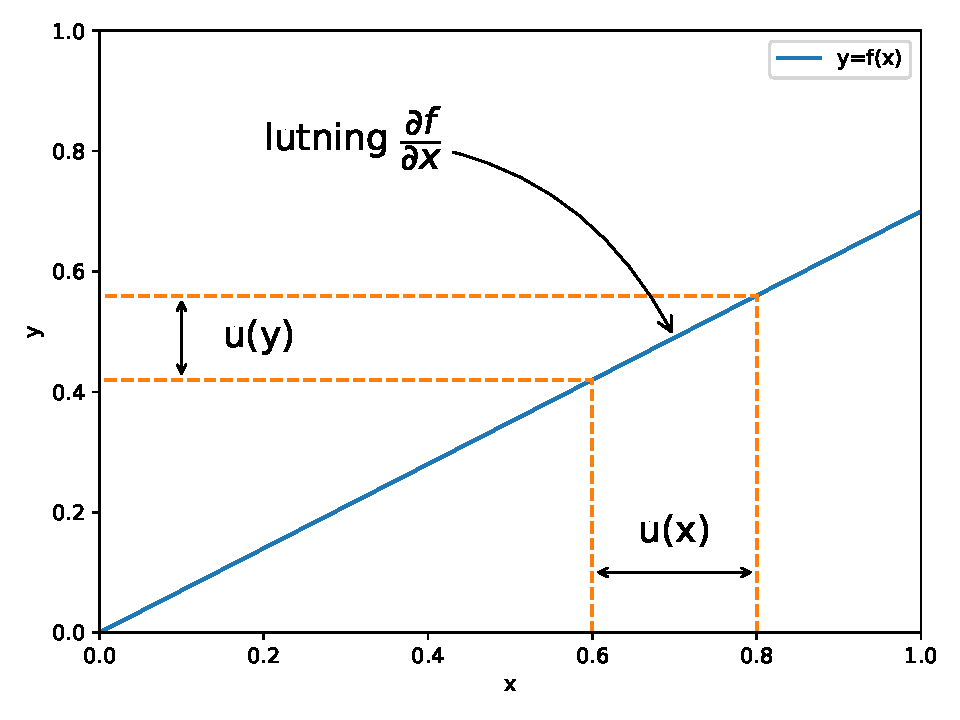
\includegraphics[width=\textwidth]{errprop1.pdf}\\
                $\frac{\partial f}{\partial x} < 1$
            \column{.5\textwidth}
                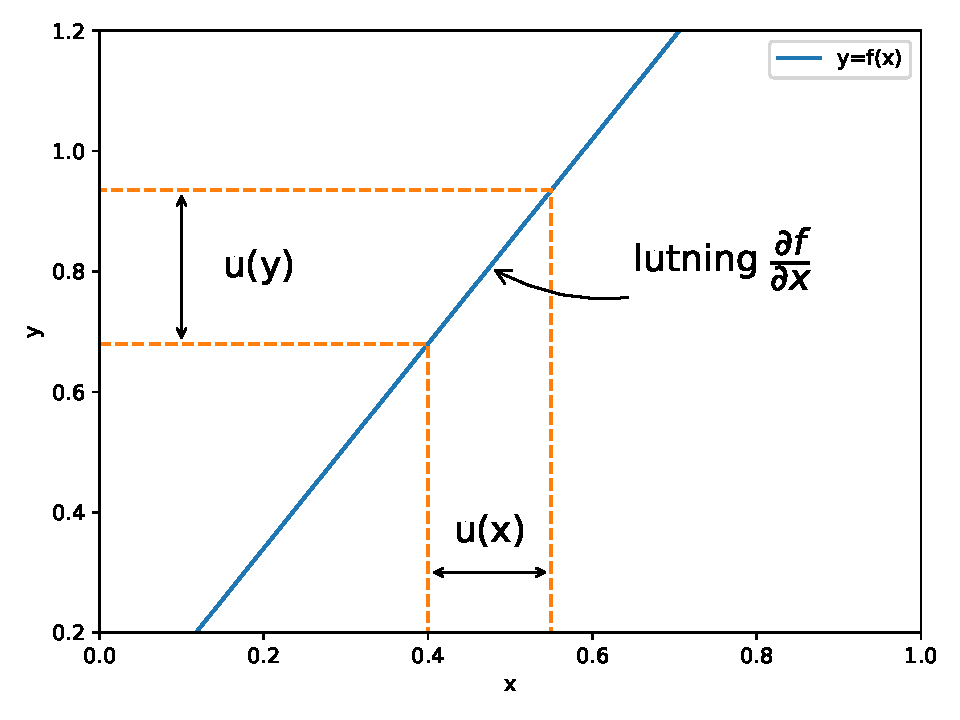
\includegraphics[width=\textwidth]{errprop2.pdf}\\
                $\frac{\partial f}{\partial x} > 1$
        \end{columns}
    \end{frame}


    \begin{frame}
        Exempel: Volymen $V$ av en cylinder beror på radien $r$ och höjden $h$
        \begin{equation*}
            V(r, h) = \pi r^2 h
        \end{equation*}
        Hur relaterar mätosäkerheter i $r$ och $h$ till mätosäkerheten i $V$? 
        \begin{equation*}
            u(y) = \sqrt{\sum_{i=1}^n\left(u(x_i)\frac{\partial f}{\partial x_i}\right)^2}
        \end{equation*}
        \begin{equation*}
             \frac{\partial V}{\partial r} = 2\pi r h, \quad \frac{\partial V}{\partial h} = \pi r^2
        \end{equation*}
        Detta ger att
        \begin{align*}
            u_V &= \sqrt{\left(u_r\frac{\partial V}{\partial r}\right)^2 + \left(u_h\frac{\partial V}{\partial h}\right)^2} =
            \sqrt{(u_r 2\pi r h)^2 + (u_h \pi r^2)^2} \\
            &= \pi r^2 h \sqrt{4\left(\frac{u_r}{r}\right)^2 + \left(\frac{u_h}{h}\right)^2}
            = V \sqrt{4\left(\frac{u_r}{r}\right)^2 + \left(\frac{u_h}{h}\right)^2}
        \end{align*}
        dvs den relativa mätosäkerheten är
        \begin{align*}
            \frac{u_V}{V} = \sqrt{4\left(\frac{u_r}{r}\right)^2 + \left(\frac{u_h}{h}\right)^2}
        \end{align*}

    \end{frame}

    \begin{frame}
        \begin{center}
            \huge{Återkommande intervall}
        \end{center}
    \end{frame}

    \begin{frame}
        \onslide<+->
        Exempel: Periodtiden för en pendel kan mätas genom att anteckna tiden $t_i$ vid varje fullbordad svängning.
        Detta ger mätserien $\{t_1, \ldots, t_i, \ldots, t_n\}$. Det är då lockande ta medelvärdet av
        $\Delta t_i = t_{i+1} - t_{i}$:
        \begin{equation*}
            \mean{t} = \frac1n \sum_i \Delta t_i = \frac{t_2 - t_1 + t_3 - t_2 + \ldots + t_{n-1} - t_{n-2} + t_n - t_{n-1}}{n} = \frac{t_n - t_1}{n}
        \end{equation*}
        dvs hur många mätningar vi än gör använder vi bara den första och sista!\\
        $\rightarrow$ Lösningen är metoden för \emph{återkommande intervall}.

        \vfill

        \onslide<+->
        Dela in mätningarna i $m=n/2$ intervall:
        \begin{columns}
            \column{.6\textwidth}
            \begin{align*}
                T_1 &= \frac{t_{m+1} - t_1}{m}\\
                T_2 &= \frac{t_{m+2} - t_2}{m}\\
                    &\vdots\\
                T_m &= \frac{t_{2m} - t_m}{m}\\
            \end{align*}
            \column{.4\textwidth}
            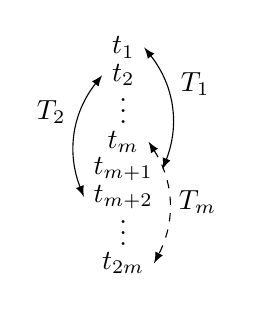
\begin{tikzpicture}
                \coordinate (dA) at (0,-1em);
                \coordinate (dB) at (0,-1.4em);
                \draw (0,0) node(t1){$t_1$}
                ++(dA)node(t2){$t_2$}
                ++(dA)node{\vdots}
                ++(dB)node(tm){$t_m$}
                ++(dA)node(tm1){$t_{m+1}$}
                ++(dA)node(tm2){$t_{m+2}$}
                ++(dA)node{\vdots}
                ++(dB)node(t2m){$t_{2m}$};
                \draw[bend left,<->,>=latex] (t1.east) to node [auto] {$T_1$} (tm1.east);
                \draw[bend right,<->,>=latex] (t2.west) to node [auto,anchor=south east] {$T_2$} (tm2.west);
                \draw[bend left,<->,dashed,>=latex] (tm.east) to node [auto] {$T_m$} (t2m.east);
            \end{tikzpicture}
            $T_i = \frac{t_{m+i} - t_i}{m}$
        \end{columns}
    Medelvärde och osäkerheter kan då beräknas med den nya mätserien $\{T_i\}_{i=1}^m$.
    \end{frame}

    \begin{frame}[fragile]
        I Matlab:
        \begin{minted}[frame=leftline,framesep=2mm,autogobble,escapeinside=||]{matlab}
        t = [1.06 2.01 2.98 3.96 5.02 6.02]; % mätdata |$t_i$|
        m = length(t)/2; % mittpunkten av mätserien |$m$|
        
        % övre och undre halvan av mätserien
        t_below = t(1:m);
        t_above = t(m+1:end);
        
        % frekvensen enligt formeln för återkommande intervall
        T = (t_above - t_below) / m;
        
        % medelvärdet och dess osäkerhetet beräknas som vanligt
        mT = mean(T);
        umT = std(T)/sqrt(m);
        \end{minted}

        \vfill
        Ovanstående exempel ger
        \begin{equation*}
            \mean{T} = \SI{0.994\pm0.014}{s}
        \end{equation*}
    \end{frame}






    % \begin{frame}
    %     Exempel: Periodtiden för en pendel ges av $T = 2\pi\sqrt{L/g}$ vilket ger ett uttryck för gravitationskonstanten $g$:
    %
    %     \begin{equation*}
    %         g = f(L, T) = \frac{4\pi^2L}{T^2}
    %     \end{equation*}
    %
    %     Detta ger
    %     \begin{equation*}
    %         \frac{\partial f}{\partial L} = \frac{4\pi^2}{T^2}\quad,\quad\frac{\partial f}{\partial T} = -2\frac{4\pi^2L}{T^3}\\
    %     \end{equation*}
    %
    %     \begin{align*}
    %         u(g) &= \sqrt{u(L)^2\left(\frac{4\pi^2}{T^2}\right)^2 + u(T)^2\left(-2\frac{4\pi^2L}{T^3}\right)^2} \\
    %             &= \frac{4\pi^2}{T^2} \sqrt{u(L)^2 + u(T)^2\frac{4L^2}{T^2}}
    %     \end{align*}
    %
    %     Vi antar här att vi redan känner till $u(L)$ och $u(T)$.
    % \end{frame}



    \begin{frame}
        Studentportalen/DOKUMENT/Laborationer/Datorlabb
        \begin{itemize}
            \item matvarden.pdf
            \item Kompendium.pdf
            \item Sammanfattning.pdf
            \item lektionsuppgift.pdf
        \end{itemize}
    \end{frame}

    \fullpage{Bonus}

    \backupbegin
    
     \begin{frame}
        \onslide<+->
        Vi säger att en slumpvariabel $X$ följer en sannolikhetsfördelning (pdf) $p(x)$ om
        \begin{equation*}
            P(x < X < x + dx) = p(x)dx
        \end{equation*}
        dvs sannolikheten att $X$ faller inom intervallet $(x, x+dx)$ är $p(x)dx$.

        \vfill

        \onslide<+->
        \begin{columns}
            \column{.5\textwidth}
        Funktionen $p(x)$ har egenskapen
        \begin{equation*}
            \int_\Omega p(x)dx = 1
        \end{equation*}
        där $\Omega$ är utfallsrummet, dvs alla möjliga värden av $X$.
            \column{.5\textwidth}
            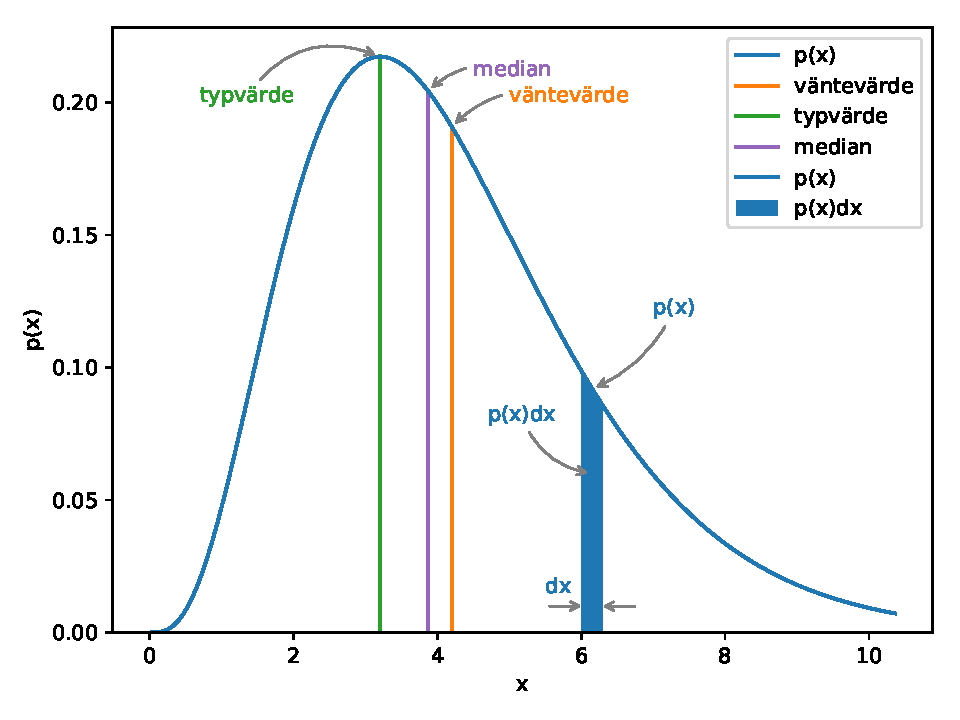
\includegraphics[width=\textwidth]{pdf.pdf}
        \end{columns}

        \vfill

        \onslide<+->
        Två viktiga koncept är
        \begin{itemize}
            \item Väntevärdet: $\mu = E[x] = \int_\Omega x p(x) dx$
                \begin{itemize}
                    \item Väntevärdet $\neq$ typvärdet (troligaste värdet) generellt! Likhet endast för \emph{symmetriska} fördelningar
                \end{itemize}
            \item Standardavvikelsen: $\sigma = \sqrt{E[(x - \mu)^2]} = \sqrt{\int_\Omega (x - \mu)^2p(x)dx}$
                \begin{itemize}
                    \item Ibland används istället variansen $V[x] = \sigma^2$
                \end{itemize}
        \end{itemize}
    \end{frame}
    
    \begin{frame}
        \begin{columns}[T]
            \column{.5\textwidth}
                Riktighet
                \vfill
                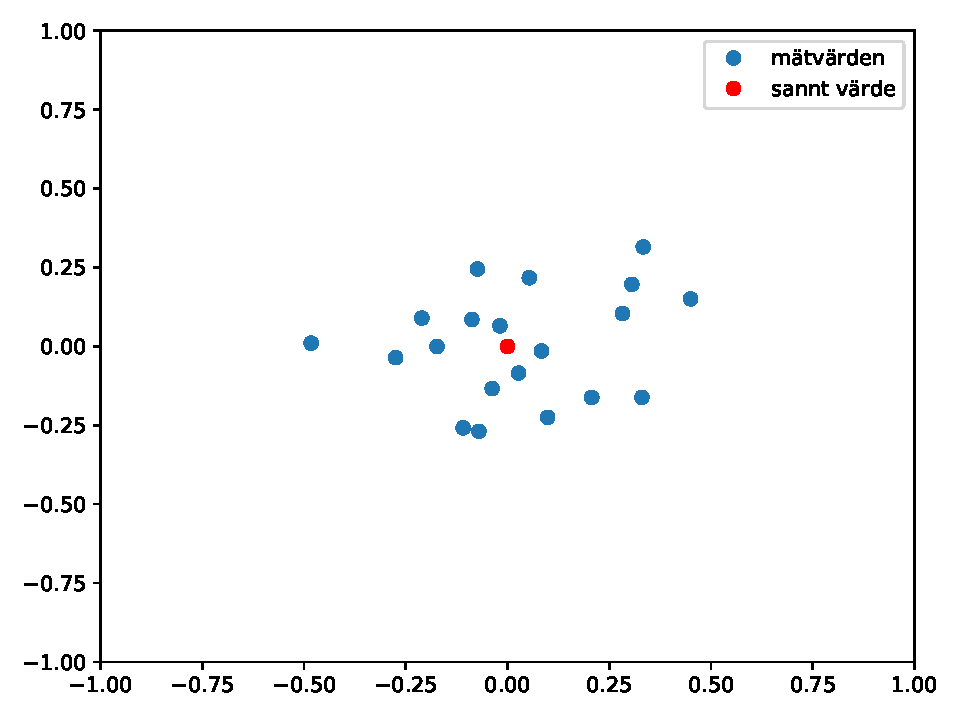
\includegraphics[width=\textwidth]{riktighet.pdf}
                \begin{itemize}
                    \item Medelvärdet $\mean{x}$ nära det sanna värdet $\mu$
                    \item Spridningen kan vara stor
                    \item Osäkerheten kan förbättras med mer data
                \end{itemize}
            \column{.5\textwidth}
                Precision
                \vfill
                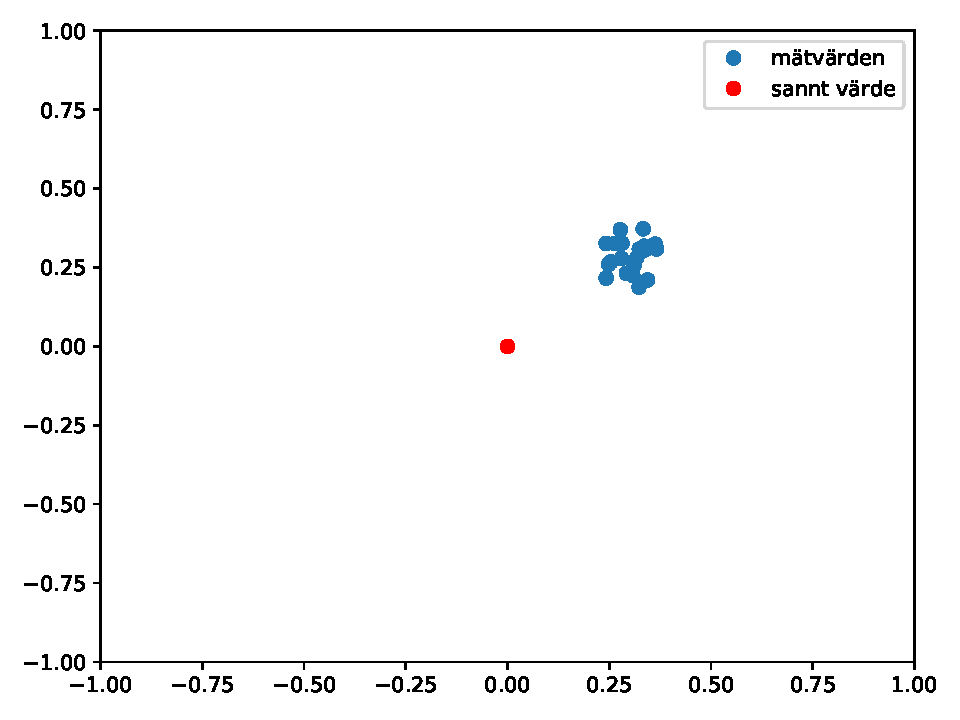
\includegraphics[width=\textwidth]{precision.pdf}
                \begin{itemize}
                    \item Medelvärdet $\mean{x}$ kan skilja sig från det sanna värdet $\mu$
                    \item Liten spridning $u(x)$
                    \item Systematiska fel som kan korrigeras
                \end{itemize}
        \end{columns}

        \vfill

        I experiment vill man ha hög riktighet (välkalibrerad utrustning) och
        hög precision (många mätningar) $\rightarrow$ Hög \emph{noggrannhet}
        (riktighet + precision)!
    \end{frame}

    \begin{frame}
        Om osäkerheten för ett mätvärde $x$ kommer från flera \emph{oberoende} källor måste dessa adderas kvadratiskt
        \begin{equation*}
            u(x) = \sqrt{\sum_i u_i^2}
        \end{equation*}

        Exempelvis om $x$ är en mätning av en sträcka $x=l_1 - l_0$ finns en avläsningsosäkerhet i både $l_1$ och $l_0$, så
        \begin{equation*}
            u(x) = \sqrt{u_0^2 + u_1^2}
        \end{equation*}

        \begin{columns}
            \column{.5\textwidth}
            \begin{tikzpicture}
                \draw (0,0) node{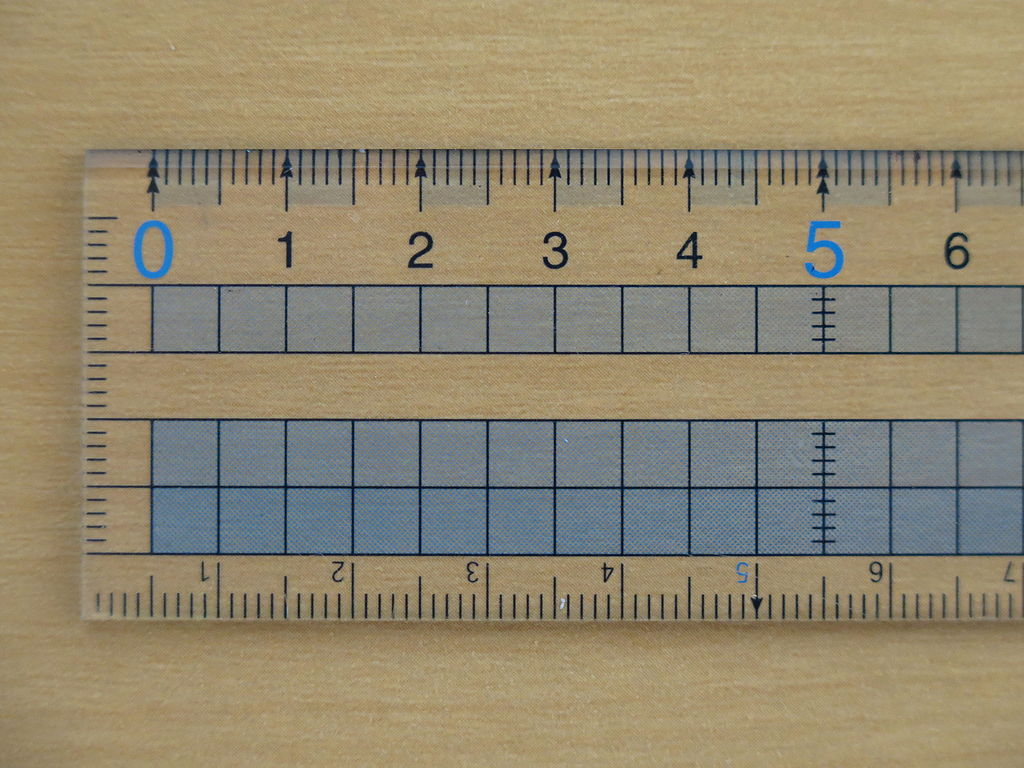
\includegraphics[width=0.9\textwidth]{Ruler_on_table.jpg}};
                % \draw[thick,red!80!black,->] (-18mm,13mm) node[align=center, above]{$l_0$} -- (-17mm,11mm);
                % \draw[thick,red!80!black,->] (16mm,13mm) node[align=center, above]{$l_1$} -- (15mm,11mm);
                \draw[very thick,red!80,->,>=latex] (-12mm,1mm) node[outer sep=0, align=center, below, fill=red!80, fill opacity=0.6, text opacity=1, rounded corners=2mm, text=black]{{\huge$l_0\pm u_0$}} -- (-17mm,11mm);
                \draw[very thick,red!80,->,>=latex] (10mm,1mm) node[outer sep=0, align=center, below, fill=red!80, fill opacity=0.6, text opacity=1, rounded corners=2mm, text=black]{{\huge$l_1\pm u_1$}} -- (15mm,11mm);
            \end{tikzpicture}
            \column{.5\textwidth}
            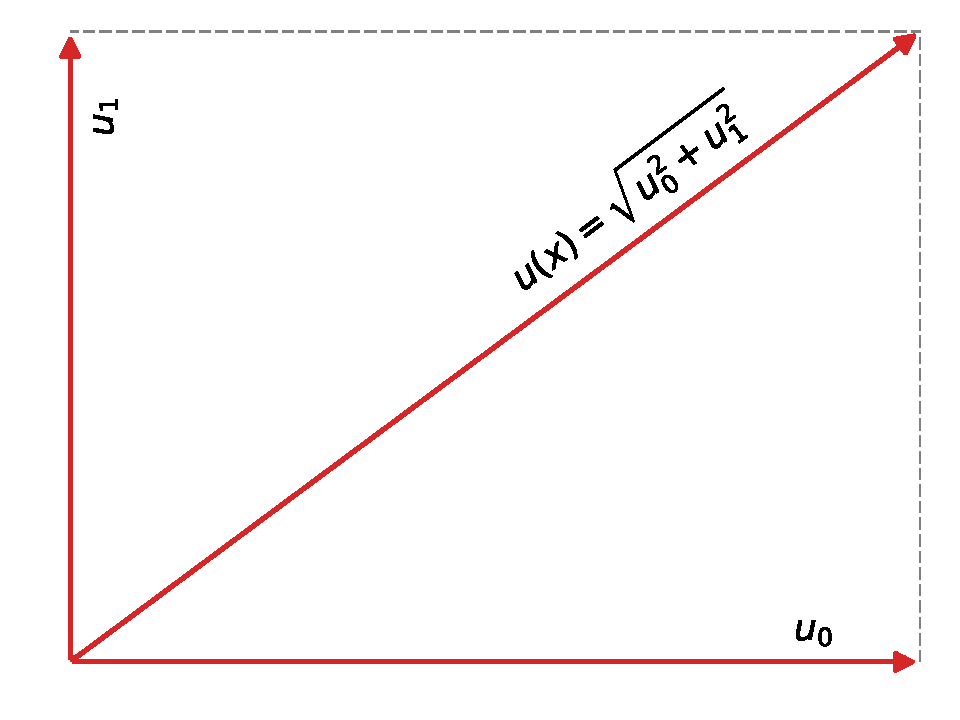
\includegraphics[width=\textwidth]{sammanlaggning.pdf}
        \end{columns}
    \end{frame}

    \begin{frame}
        Exempel: Anpassa en konstant $a$ till en mätserie $\{x_i\}$.
        \begin{columns}[T]
            \column{.5\textwidth}
            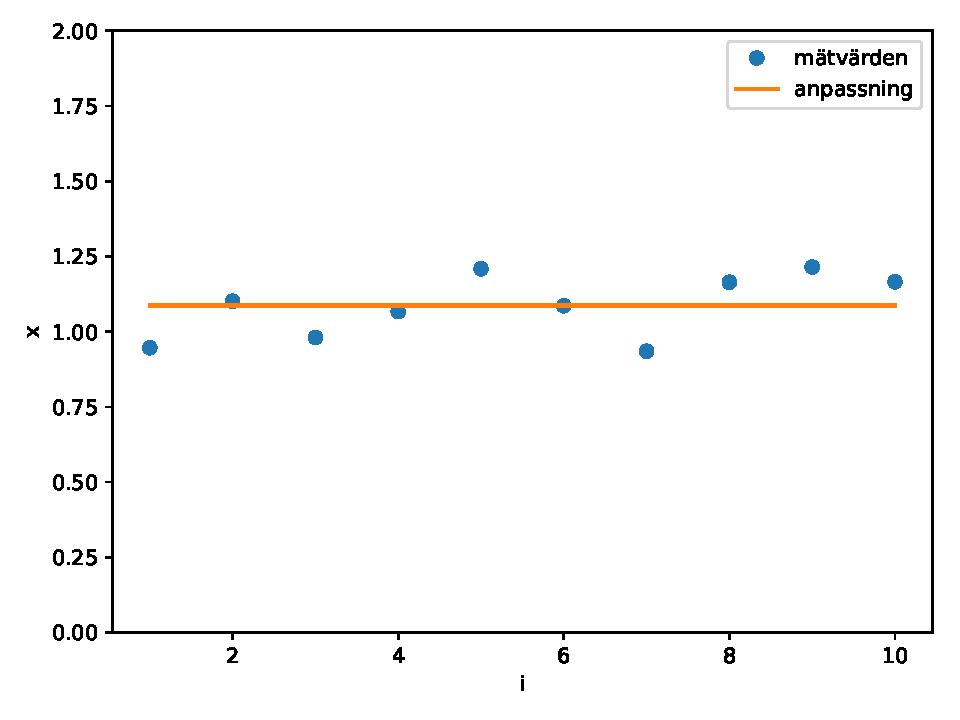
\includegraphics[width=\textwidth]{anpassning1.pdf}
            \column{.5\textwidth}
            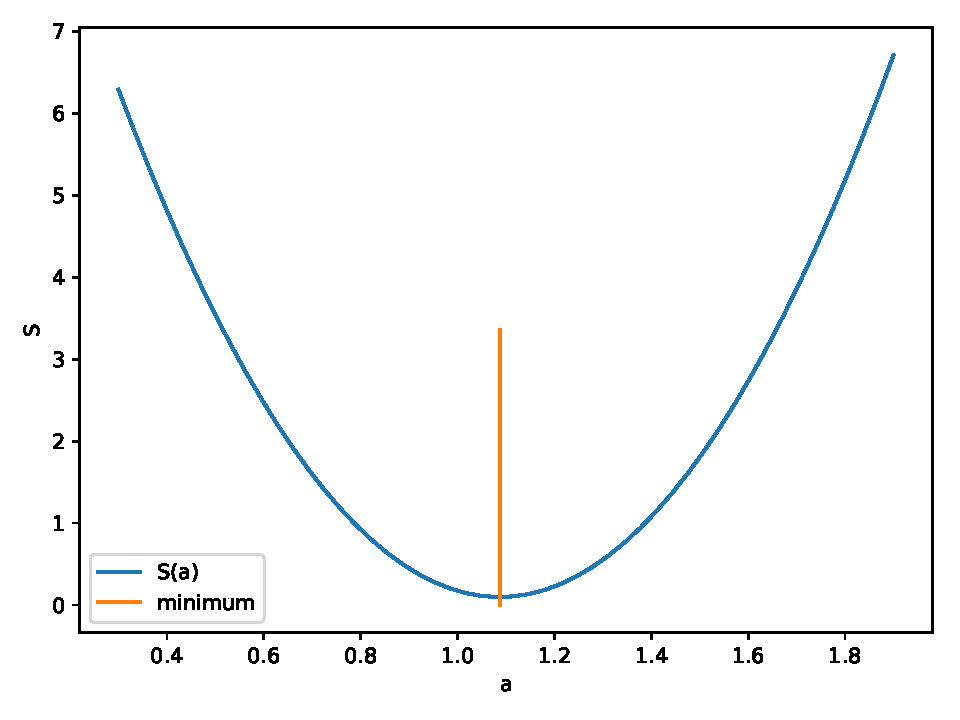
\includegraphics[width=\textwidth]{s1.pdf}
        \end{columns}

        Bilda kvadratsumman $S$ och derivera:
        \begin{gather*}
        S(a) = \sum_i (x_i - a)^2\quad\rightarrow\quad\frac{\partial S}{\partial a} = -2\sum_i(x_i-a) = \left(-2\sum_ix_i\right) +2na\right) = 0\\
             \rightarrow\quad na = \sum_i x_i\quad
                                       \rightarrow\quad a = \frac1n\sum_i x_i = \mean{x}
        \end{gather*}
        Så medelvärdet $\mean{x}$ är den konstant som passar vår data bäst!
        Här blir $a=1.09$, medan det sanna värdet var 1.10.
    \end{frame}

    \begin{frame}
        Om mätvärdena $y_i$ har en associerad mätosäkerhet $u_i$ måste dessa tas hänsyn till.

        \vfill
        Detta görs genom att vikta varje term i kvadratsumman $S$ med sin mätosäkerhet

        \vfill
        \begin{columns}
            \column{.5\textwidth}
            \begin{equation*}
                S = \sum_i \frac{(y_i - f(x_i, \vec a))^2}{u_i^2}
            \end{equation*}
            och därefter fortsätta som vanligt, dvs genom att lösa
            \begin{equation*}
                \frac{\partial S}{\partial a_j} = -2\sum_i \frac{y_i - f(x_i, \vec a)}{u_i^2}\frac{\partial f(x_i, \vec a)}{\partial a_j} = 0
            \end{equation*}
            för varje parameter $a_j$.
            \column{.5\textwidth}
            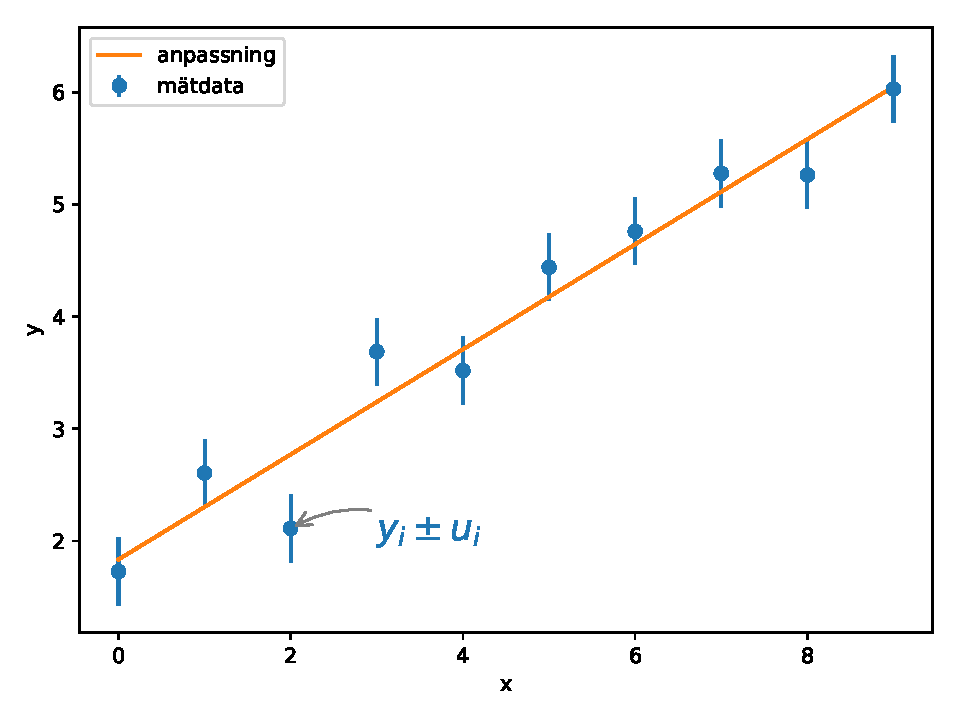
\includegraphics[width=\textwidth]{anpassning3.pdf}
        \end{columns}

    \end{frame}

    \begin{frame}
        \textbf{OBS!} Allt som följer nu ingår \emph{inte} i kursen utan är endast till för den intresserade :)
        \vfill
        Linjär minstakvadratanpassning kan skrivas helt med hjälp av matriser, vilket ger en väldigt kompakt notation. Detta lämpar sig också väl för Matlab och dylikt.
        \vfill

        Definiera $\vec x$, $\vec y$, och $\vec a$ som vanligt:
        \begin{equation*}
            \vec x = (x_1, \ldots, x_n)^\top\quad \vec y = (y_1, \ldots, y_n)^\top \quad \vec a = (a_1,\ldots,a_m)^\top
        \end{equation*}
        Vi behöver två matriser till, designmatrisen $X$ och kovariansmatrisen $\Sigma$:
        \begin{equation*}
            X = \begin{pmatrix}
                1      & x_1    & x_1^2    & \ldots & x_1^{m-1} \\
                1      & x_2    & x_2^2    & \ldots & x_2^{m-1} \\
                \vdots & \vdots & \vdots   & \ddots & \vdots    \\
                1      & x_n    & x_n^2    & \ldots & x_n^{m-1} \\
            \end{pmatrix},\quad
            \Sigma = \mathrm{diag}\{u_i^2\} = \begin{pmatrix}
                u_1^2 & 0 & \ldots & 0 \\
                0 & u_2^2 & \ldots & 0 \\
                \vdots & \vdots & \ddots & \vdots \\
                0 & 0 & \ldots & u_n^2 \\
            \end{pmatrix}\\
        \end{equation*}
        \vfill
        Observera att formen på $X$ ovan endast gäller för anpassning av polynom, $f(x) = a_1 + a_2x + a_3x^2 + \ldots + a_mx^{m-1}$.
    \end{frame}

    \begin{frame}
        Kvadratsummas $S$ kan då skrivas som
        \begin{equation*}
            \quad S = \left(\vec y - X \vec a\right)^\top\Sigma^{-1}\left(\vec y - X \vec a\right)\\
        \end{equation*}
        Vi kan nu derivera $S$ med avseende på \emph{vektorn}%
        \footnote{\url{https://en.wikipedia.org/wiki/Matrix_calculus}}%
        \footnote{\url{https://www.math.uwaterloo.ca/~hwolkowi/matrixcookbook.pdf}}
         $\vec a$
        \begin{equation*}
            \frac{\partial S}{\partial \vec a} = -2X^\top\Sigma^{-1}\left(\vec y - X\vec a\right) = 0
        \end{equation*}
        Efter lite omordning får vi då
        \begin{gather*}
            X^\top\Sigma^{-1} \vec y = X^\top\Sigma^{-1} X \vec a\\
            \vec a = \left(X^\top \Sigma^{-1} X\right)^{-1}X^\top \Sigma^{-1} \vec y
        \end{gather*}
        vilket direkt ger parametrarna $\vec a$!
    \end{frame}

    \begin{frame}
        Även mätosäkerheterna i $\vec a$ kan skrivas på matrisform. Notera att vi har
        \begin{equation*}
            \vec a = \left(X^\top \Sigma^{-1} X\right)^{-1}X^\top \Sigma^{-1} \vec y
        \end{equation*}
        Vi kan då ta derivatan av $\vec a$ med avseende på $\vec y$%
        \footnote{\url{https://en.wikipedia.org/wiki/Matrix_calculus}}%
        \footnote{\url{https://www.math.uwaterloo.ca/~hwolkowi/matrixcookbook.pdf}}
        \begin{equation*}
            \mathcal J \equiv \frac{\partial \vec a}{\partial \vec y} = \left(X^\top \Sigma^{-1} X\right)^{-1}X^\top \Sigma^{-1}
        \end{equation*}
        Matrisen $\mathcal J$ kallas för Jacobianen för $\vec a$ med avseende på $\vec y$ och är analog med derivatan för vanliga funktioner. Mätosäkerheterna fås då med felpropagering som på matrisform är
        \begin{equation*}
            \Sigma_a = \mathcal J \Sigma \mathcal J^\top = \text{[algebra]} = \left(X^\top\Sigma^{-1}X\right)^{-1}
        \end{equation*}
        där $\Sigma_a$ är kovariansmatrisen för $\vec a$. Mätosäkerheterna fås då som roten ur diagonalelementen
        \begin{equation*}
            \vec u_a = \sqrt{\mathrm{diag}\left(\Sigma_a\right)}
        \end{equation*}
        och vi är klara!
    \end{frame}

    \begin{frame}[fragile]
        I Matlab tar allt ovanstående den relativt kompakta formen:
        \begin{minted}[frame=leftline,framesep=2mm,autogobble,escapeinside=||]{matlab}
            % mätdata |$\{x_i, y_i \pm u_i\}$| som kolonnvektorer
            x = [|\ldots|]'; y = [|\ldots|]'; u = [|\ldots|]';
            X = [x.^0, x.^1, |\ldots|]; % designmatrisen |$X$|

            % kovariansmatrisen |$\Sigma$|, samt inversen |$\Sigma^{-1}$|
            V = diag(u.^2); iV = inv(V);
            J = inv(X'*iV*X)*X'*iV; % Jacobianen |$\mathcal{J}$|
            a = J*y; % de anpassade parametrarna |$a$|
            Va = J*V*J' % kovariansmatrisen |$\Sigma_a$|
            ua = sqrt(diag(Va)); % mätosäkerheter |$u_a$|
        \end{minted}
    \end{frame}

    \backupend

\end{document}
